%% FullCourse_10Lecs -- Lecture 1, Topic 1.3b: The AI/RL Alternative
%% Source: ./archive_pre_split/Lec01_Quant_Macro.tex (section 6)
%% Pass A mechanical split (verbatim content preserved).
%% Sub-split sibling of T3a (Extensions §5).

%% Shared preamble for the FullCourse_10Lecs topic decks.
%%
%% Each topic .tex \input's this file, then defines its own \title, \date
%% override (if any), \graphicspath, and \begin{document}.
%%
%% Reconstructed verbatim from the inlined copy preserved in
%% Lec10_Case_Studies/Lec10_T8_Case6_DeepRamsey.tex (lines 23-190), which is
%% explicitly annotated there as "from ../shared_preamble.tex, copied verbatim".
%% Base preamble matches MiniCourse_8hr/Slides/shared_preamble.tex; this version
%% additionally provides \sectiondivider, the conceptbox/cautionbox/examplebox/
%% takeawaybox tcolorboxes, and \compacttables used across the split decks.

\documentclass[10pt,english,aspectratio=169]{beamer}

\usepackage{ae,aecompl}
\usepackage[T1]{fontenc}
\usepackage{textcomp}
\usepackage[utf8]{inputenc}
\usepackage{babel}
\usepackage{datetime2}

\setcounter{secnumdepth}{3}
\setcounter{tocdepth}{3}

\usepackage{amsmath, amssymb, amsthm, graphicx}
\usepackage{booktabs, multirow}
\usepackage{tikz}
\usepackage{pgfplots}
\pgfplotsset{compat=1.16}
\usepackage[most]{tcolorbox}
\tcbuselibrary{skins, breakable, theorems}
\usepackage{listings}
\usepackage{xcolor}

\lstset{
  basicstyle=\ttfamily\small,
  keywordstyle=\color{blue!80!black}\bfseries,
  commentstyle=\color{green!50!black}\itshape,
  stringstyle=\color{orange!80!black},
  backgroundcolor=\color{gray!8},
  frame=single,
  rulecolor=\color{gray!40},
  breaklines=true,
  showstringspaces=false,
  numbers=none,
}

\lstdefinestyle{pythonstyle}{
    language=Python,
    basicstyle=\ttfamily\footnotesize,
    keywordstyle=\color{blue!80!black}\bfseries,
    commentstyle=\color{green!50!black}\itshape,
    stringstyle=\color{orange!80!black},
    frame=single,
    breaklines=true,
    showstringspaces=false,
    numbers=left,
    numbersep=5pt,
    numberstyle=\tiny\color{gray},
    backgroundcolor=\color{gray!8},
    rulecolor=\color{gray!40}
}

\ifx\hypersetup\undefined
  \AtBeginDocument{%
    \hypersetup{bookmarks=false,breaklinks=true,pdfborder={0 0 0},colorlinks=true,
      linkcolor=DarkText,urlcolor=RedTitle}%
  }
\else
  \hypersetup{bookmarks=false,breaklinks=true,pdfborder={0 0 0},colorlinks=true,
    linkcolor=DarkText,urlcolor=RedTitle}%
\fi

\makeatletter
\newcommand\makebeamertitle{%
  \begin{frame}[plain]
    \vspace*{1.0cm}
    \centering
    {\usebeamerfont{title}\usebeamercolor[fg]{title}\inserttitle\par}
    \vspace{1.0cm}
    {\usebeamerfont{author}\usebeamercolor[fg]{author}\insertauthor\par}
    \vspace{0.2cm}
    {\usebeamerfont{date}\usebeamercolor[fg]{date}\insertdate\par}
  \end{frame}}%
\AtBeginDocument{%
  \let\origtableofcontents=\tableofcontents
  \def\tableofcontents{\@ifnextchar[{\origtableofcontents}{\gobbletableofcontents}}
  \def\gobbletableofcontents#1{\origtableofcontents}%
}

\usetheme{metropolis}
\usefonttheme{professionalfonts}

\definecolor{LightGray}{RGB}{230,230,230}
\definecolor{RedTitle}{RGB}{0,0,200}
\definecolor{VeryLightGray}{RGB}{245,245,245}
\definecolor{DarkText}{RGB}{0,0,0}

\setbeamercolor{background canvas}{bg=white}
\setbeamercolor{title}{fg=RedTitle}
\setbeamercolor{author}{fg=DarkText}
\setbeamercolor{date}{fg=DarkText}
\setbeamercolor{frametitle}{bg=VeryLightGray,fg=DarkText}
\setbeamercolor{normal text}{fg=DarkText}
\setbeamerfont{title}{size=\large}

\setbeamersize{text margin left=5mm, text margin right=5mm}
\addtobeamertemplate{frametitle}{}{\vspace{-0.5em}}
\newcommand{\reducevspace}{\vspace{-0.5cm}}

% Shared section divider and box styles for split topic decks.
\newcommand{\sectiondivider}[2]{%
\begin{frame}[plain,noframenumbering]
\begin{center}
\vfill
{\Large\textbf{#1}\par}
\vspace{0.35cm}
{\normalsize #2\par}
\vfill
\end{center}
\end{frame}
}

\newtcolorbox{conceptbox}[1][]{
  colback=blue!3,
  colframe=RedTitle!55,
  boxrule=0.35mm,
  arc=1mm,
  left=2mm,
  right=2mm,
  top=1mm,
  bottom=1mm,
  #1
}
\newtcolorbox{cautionbox}[1][]{
  colback=red!3,
  colframe=red!50!black,
  boxrule=0.35mm,
  arc=1mm,
  left=2mm,
  right=2mm,
  top=1mm,
  bottom=1mm,
  #1
}
\newtcolorbox{examplebox}[1][]{
  colback=green!3,
  colframe=green!45!black,
  boxrule=0.35mm,
  arc=1mm,
  left=2mm,
  right=2mm,
  top=1mm,
  bottom=1mm,
  #1
}
\newtcolorbox{takeawaybox}[1][]{
  colback=VeryLightGray,
  colframe=RedTitle!55,
  boxrule=0.35mm,
  arc=1mm,
  left=2mm,
  right=2mm,
  top=1mm,
  bottom=1mm,
  #1
}
\newcommand{\compacttables}{\renewcommand{\arraystretch}{1.15}}

\setbeamertemplate{navigation symbols}{}
\setbeamertemplate{footline}{%
  \hfill%
  \usebeamercolor[fg]{page number in head/foot}%
  \usebeamerfont{page number in head/foot}%
  \insertframenumber\,/\,\inserttotalframenumber\kern1em\vskip2pt%
}

\makeatother

\author{Zhigang Feng}
% "date with time": compile timestamp so each build is identifiable.
\date{\today\ \DTMcurrenttime}


\graphicspath{{./pic/}{../../FullCourse_10Lecs/Lec01_Quant_Macro/pic/}{../}}

\title[AI for Econ Research]{AI for Economic Research: Dynamic Models, Language, and Agents\\
Lecture 1.3b: The AI/RL Alternative}

\begin{document}

\makebeamertitle

%=============================================================================
\begin{frame}{Topic 1.3b Agenda}
\begin{enumerate}
  \item \textbf{The Robot-Taxi Problem} --- RL framing of dynamic programming
  \medskip
  \item \textbf{Monte Carlo, Function Approximation, Sampled Data} --- the AI toolkit
  \medskip
  \item \textbf{HA Models as Middle Ground} --- bridging two traditions
  \medskip
  \item \textbf{Numerical Techniques: Classical vs.\ AI Frontier}
  \medskip
  \item \textbf{Course Roadmap and Programming Environment}
\end{enumerate}
\end{frame}

%=============================================================================
\section{The AI/RL Alternative}

\begin{frame}{AI/Reinforcement Learning: The Robot-Taxi Problem}
\begin{itemize}
\item \textbf{Example:} Training an autonomous vehicle to navigate a city

\medskip
\item \textbf{State Space:} Camera images, LiDAR, GPS, speed, ...
\begin{itemize}
    \item Single camera frame: $1920 \times 1080 \times 3 \approx 6$ million dimensions
    \item Continuous, high-dimensional, partially observable
\end{itemize}

\medskip
\item \textbf{Action Space:} Steering, acceleration, braking (continuous)

\medskip
\item \textbf{Environment:} Transition dynamics $P(s'|s, a)$
\begin{itemize}
    \item Physics, other drivers, pedestrians, weather
    \item \emph{Unknown} and \emph{impossible to fully specify}
    \item No ``First Welfare Theorem'' to simplify
\end{itemize}

\medskip
\item \textbf{Contrast with Macro:} No closed-form model; must learn from experience
\end{itemize}
\end{frame}

\begin{frame}{RL Formulation: The Same Bellman Equation}
\begin{itemize}
\item \textbf{Markov Decision Process (MDP):} $(S, A, P, r, \beta)$

\medskip
\item \textbf{Bellman Equation for Optimal Value:}
\[
v^*(s) = \max_{a} \left\{ r(s, a) + \beta \int v^*(s') P(ds'|s, a) \right\}
\]

\medskip
\item \textbf{Bellman Equation for Q-Function:}
\[
Q^*(s, a) = r(s, a) + \beta \int \max_{a'} Q^*(s', a') P(ds'|s, a)
\]

\medskip
\item \textbf{Key Insight:} Theoretical foundation is \emph{identical} to economics.
\begin{itemize}
    \item Bellman equation, contraction mapping, fixed point---all apply
\end{itemize}

\medskip
\item \textbf{The difference is computational:} How do we solve this when $P$ is unknown and $S$ is enormous?
\end{itemize}
\end{frame}

\begin{frame}{Three Fundamental Challenges}
\begin{center}
\renewcommand{\arraystretch}{1.4}
\begin{tabular}{|c|c|c|}
\hline
\textbf{Challenge} & \textbf{Classical DP} & \textbf{Modern AI/RL} \\
\hline
\textbf{Dimensionality} & Low $(d \leq 5)$ & Very high $(d \geq 10^6)$ \\
\hline
\textbf{Environment} & Fully known & Unknown, learned \\
\hline
\textbf{Data} & Regular grids & Random samples \\
\hline
\end{tabular}
\end{center}

\bigskip
\begin{itemize}
\item \textbf{Dimensionality:} Cannot discretize; must use function approximation
\item \textbf{Unknown Environment:} Cannot evaluate $\mathbb{E}[v(s')]$ analytically; estimate from samples (Monte Carlo)
\item \textbf{Irregular Data:} Samples from trajectories, not grids; must generalize
\end{itemize}
\end{frame}

\begin{frame}{Monte Carlo: Turning Samples into Expectations}
\begin{itemize}
\item \textbf{The Problem:} Computing $\mathbb{E}[v(s') | s, a] = \int v(s') P(ds'|s, a)$
\begin{itemize}
    \item Classical DP: Enumerate all $s'$, weight by known $P(s'|s, a)$
    \item High dimensions or unknown $P$: Infeasible
\end{itemize}

\medskip
\item \textbf{Monte Carlo Estimation:}
\[
\mathbb{E}[v(s')] \approx \frac{1}{N} \sum_{i=1}^{N} v(s'_i), \qquad s'_i \sim P(\cdot | s, a)
\]
\begin{itemize}
    \item Generate samples by \emph{simulating} or \emph{interacting} with environment
    \item Law of Large Numbers: Converges as $N \to \infty$
\end{itemize}

\medskip
\item \textbf{Key Advantage:} Cost scales with $N$, \emph{not} dimension
\begin{itemize}
    \item Works equally well in 2 or 2 million dimensions
    \item This is how RL escapes the curse of dimensionality
\end{itemize}
\end{itemize}
\end{frame}

\begin{frame}{Function Approximation: Learning from Irregular Data}
\begin{itemize}
\item \textbf{Classical DP:} Value function as table $\{v(s_i)\}_{i=1}^{N}$
\begin{itemize}
    \item Regular grid, pre-specified, covers entire state space
    \item Interpolation straightforward
\end{itemize}

\medskip
\item \textbf{RL with Function Approximation:}
\[
v(s) \approx v_\theta(s) = \text{NeuralNetwork}_\theta(s)
\]
\begin{itemize}
    \item Parameters $\theta$ learned from sampled data
    \item Data from trajectories: $(s_0, a_0, r_0, s_1, a_1, r_1, \ldots)$
    \item Points concentrate where policy visits (not uniform)
\end{itemize}

\medskip
\item \textbf{Challenges:}
\begin{itemize}
    \item Must generalize to unseen states
    \item Approximation errors can compound (instability)
    \item No convergence guarantee (unlike tabular DP)
\end{itemize}
\end{itemize}
\end{frame}

\begin{frame}{From Grids to Samples: A Paradigm Shift}
\begin{center}
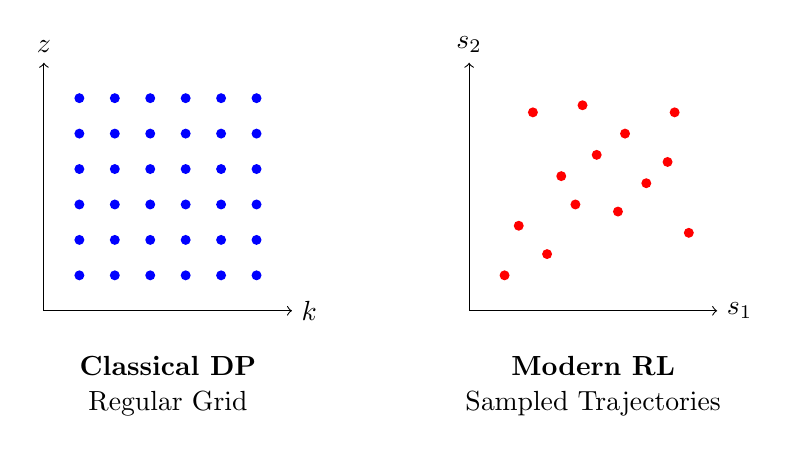
\begin{tikzpicture}[scale=0.9]
% Classical DP - Grid
\begin{scope}[shift={(-4,0)}]
\draw[->] (0,0) -- (3.5,0) node[right] {$k$};
\draw[->] (0,0) -- (0,3.5) node[above] {$z$};
\foreach \x in {0.5,1,1.5,2,2.5,3}
    \foreach \y in {0.5,1,1.5,2,2.5,3}
        \fill[blue] (\x,\y) circle (2pt);
\node[below] at (1.75,-0.5) {\textbf{Classical DP}};
\node[below] at (1.75,-1) {Regular Grid};
\end{scope}
% Modern RL - Random Samples
\begin{scope}[shift={(2,0)}]
\draw[->] (0,0) -- (3.5,0) node[right] {$s_1$};
\draw[->] (0,0) -- (0,3.5) node[above] {$s_2$};
\fill[red] (0.7,1.2) circle (2pt);
\fill[red] (1.1,0.8) circle (2pt);
\fill[red] (1.5,1.5) circle (2pt);
\fill[red] (1.3,1.9) circle (2pt);
\fill[red] (2.1,1.4) circle (2pt);
\fill[red] (1.8,2.2) circle (2pt);
\fill[red] (2.5,1.8) circle (2pt);
\fill[red] (2.2,2.5) circle (2pt);
\fill[red] (2.8,2.1) circle (2pt);
\fill[red] (0.9,2.8) circle (2pt);
\fill[red] (1.6,2.9) circle (2pt);
\fill[red] (2.9,2.8) circle (2pt);
\fill[red] (0.5,0.5) circle (2pt);
\fill[red] (3.1,1.1) circle (2pt);
\node[below] at (1.75,-0.5) {\textbf{Modern RL}};
\node[below] at (1.75,-1) {Sampled Trajectories};
\end{scope}
\end{tikzpicture}
\end{center}

\medskip
\begin{itemize}
\item \textbf{Left:} Compute $v(s)$ at every grid point; interpolate
\item \textbf{Right:} Observe $(s, a, r, s')$ tuples; fit $v_\theta(s)$ to minimize prediction error
\end{itemize}
\end{frame}

\begin{frame}{Heterogeneous Agent Models: Between Two Worlds}
\begin{itemize}
\item \textbf{Individual Problem:} Low-dimensional $(a, z)$---classical methods work
\item \textbf{Aggregate State:} Distribution $\mu$---infinite-dimensional

\medskip
\item \textbf{Traditional Approaches:}
\begin{itemize}
    \item Krusell-Smith: Approximate $\mu$ by moments $(\bar{K}, \sigma_K, \ldots)$
    \item Bounded rationality: Simple forecasting rules
    \item Iterate until forecasts approximately consistent
\end{itemize}

\medskip
\item \textbf{Modern Approaches (Research Frontier):}
\begin{itemize}
    \item Neural networks to represent policy: $g_\theta(a, z, \mu)$
    \item Monte Carlo simulation of agent distribution
    \item Learn equilibrium conditions end-to-end
\end{itemize}

\medskip
\item \textbf{Key Insight:} Heterogeneous agent macro is a middle ground---we \emph{know} economic structure but face RL-like computational challenges.
\end{itemize}
\end{frame}

\begin{frame}{Overview: Two Traditions, Shared Foundations}
\begin{center}
\renewcommand{\arraystretch}{1.3}
\begin{tabular}{|l|c|c|}
\hline
 & \textbf{Quantitative Macro} & \textbf{AI / Reinforcement Learning} \\
\hline
\textbf{Theory} & Bellman equation & Bellman equation \\
\textbf{Foundation} & Contraction mapping & Contraction mapping \\
\hline
\textbf{Environment} & Known (model-based) & Unknown (learn from data) \\
\textbf{State Space} & Low-dimensional & Very high-dimensional \\
\textbf{Computation} & Grid + interpolation & Samples + neural nets \\
\hline
\textbf{Strength} & Exploits structure & Scales to complexity \\
\textbf{Weakness} & Curse of dimensionality & Sample inefficiency \\
\hline
\end{tabular}
\end{center}

\bigskip
\textbf{The Opportunity:} Combine economic structure with ML scalability
\begin{itemize}
    \item Use theory to reduce dimensionality where possible
    \item Use neural networks where analytical solutions fail
    \item Use Monte Carlo to handle high-dimensional distributions
\end{itemize}
\end{frame}

\begin{frame}{Numerical Techniques: Classical Methods}
\begin{itemize}
\item \textbf{Function Approximation and Interpolation}
\begin{itemize}
    \item Linear/cubic splines, Chebyshev polynomials
    \item Approximating policy and value functions
\end{itemize}

\medskip
\item \textbf{Numerical Optimization}
\begin{itemize}
    \item Newton-Raphson, gradient descent, grid search
    \item Finite differences, automatic differentiation (PyTorch)
\end{itemize}

\medskip
\item \textbf{Stochastic Process Approximation}
\begin{itemize}
    \item Tauchen, Rouwenhorst methods for discretizing AR(1)
\end{itemize}

\medskip
\item \textbf{Perturbation and Projection}
\begin{itemize}
    \item Linearization around steady state
    \item Higher-order perturbation (2nd/3rd order for risk)
    \item Projection methods with basis functions
\end{itemize}
\end{itemize}
\end{frame}

\begin{frame}{Numerical Techniques: The AI Frontier}
\begin{itemize}
\item \textbf{Deep Neural Networks}
\begin{itemize}
    \item Universal approximators for high-dimensional functions
    \item Policy networks $\pi_\theta(s)$, value networks $v_\theta(s)$
\end{itemize}

\medskip
\item \textbf{Monte Carlo and Simulation}
\begin{itemize}
    \item Estimating expectations without discretization
    \item Variance reduction techniques
\end{itemize}

\medskip
\item \textbf{Stochastic Optimization}
\begin{itemize}
    \item SGD, Adam, and variants
    \item Training on mini-batches of sampled data
\end{itemize}

\medskip
\item \textbf{Reinforcement Learning}
\begin{itemize}
    \item Q-learning, policy gradient, actor-critic
    \item Solving DP when environment is unknown or complex
\end{itemize}

\medskip
\item \textbf{Adaptive Methods:} Sparse grids, active learning for efficient sampling
\end{itemize}
\end{frame}

\begin{frame}{What This Course Will Explore}
\begin{itemize}
\item \textbf{Classical Foundations:}
\begin{itemize}
    \item Dynamic programming theory (existence, uniqueness, convergence)
    \item Numerical methods: VFI, PFI, Euler iteration, projection, perturbation
\end{itemize}

\medskip
\item \textbf{Machine Learning Tools:}
\begin{itemize}
    \item Function approximation with neural networks
    \item Monte Carlo methods and variance reduction
    \item Stochastic optimization (SGD, Adam)
\end{itemize}

\medskip
\item \textbf{Bridging the Gap:}
\begin{itemize}
    \item Deep learning for solving Bellman equations
    \item Neural network solutions to heterogeneous agent models
    \item Exploiting economic structure in ML architectures
\end{itemize}

\medskip
\item \textbf{Goal:} Equip you to work at the frontier where economic theory meets computational innovation.
\end{itemize}
\end{frame}

\begin{frame}[fragile]{Programming Environment}
\begin{itemize}
\item \textbf{Python}
\begin{itemize}
    \item High-level, readable, vast ecosystem (NumPy, SciPy, Pandas)
    \item Excellent for prototyping; vectorized libraries for speed
\end{itemize}

\medskip
\item \textbf{PyTorch}
\begin{itemize}
    \item GPU-accelerated tensor computing
    \item Dynamic computational graphs with automatic differentiation
    \item Essential for modern high-dimensional solving
\end{itemize}

\medskip
\item \textbf{Quick Start:}
\begin{lstlisting}[language=Python]
import torch
import torch.nn as nn

v_net = nn.Sequential(
    nn.Linear(2, 64), nn.Tanh(),
    nn.Linear(64, 64), nn.Tanh(),
    nn.Linear(64, 1)
)
\end{lstlisting}
\end{itemize}
\end{frame}

\begin{frame}{Summary: The Big Picture}
\begin{enumerate}
\item \textbf{Theory:} Bellman equation + contraction mapping = foundation for both economics and AI

\medskip
\item \textbf{Classical Macro:} Exploits known structure; limited by dimensionality

\medskip
\item \textbf{Competitive Equilibrium:} Defined by optimality + market clearing; simplified by representative agent

\medskip
\item \textbf{Heterogeneous Agents:} Distribution as state breaks classical methods

\medskip
\item \textbf{Calibration \& Estimation:} Tie the model to data; SMM and Bayesian methods

\medskip
\item \textbf{Accuracy:} Always check Euler equation residuals; $|\text{EEE}| < 10^{-4}$ is the target

\medskip
\item \textbf{Modern AI/RL:} Scales via Monte Carlo + neural networks; sample-intensive

\medskip
\item \textbf{The Opportunity:} Combine economic structure with ML scalability
\end{enumerate}

\bigskip
\begin{center}
\textbf{This course: Learn to work at the intersection.}
\end{center}
\end{frame}

\end{document}
